\section{Optimal Mechanisms with Efficiency and Only Seller's Cost}
\label{sec:efficient}

In this section, we make two simplifying assumptions: (1) we restrict
attention to mechanisms that allocate the item efficiently and (2) we
assume that the bidder cost for replying ($\beta_2$) is zero.\footnote{Note
that if (2) does not hold, then allocating efficiently may not be possible
without the seller compensating the bidders for their bid costs.}
%we consider a simplified optimizing problem with efficiency
%constraint and only seller's cost.  Though these two constraints simplify our
%problem a lot, they are reasonable in real cases such as craigslist or moving
%sales in mailing-lists. 
For example, someone who is moving and selling furniture on craigslist is
likely to have $0$ valuation for the item 
and cannot commit to withhold the item or prevent re-sale between
bidders. Under such circumstances,  efficient mechanisms not only maximizes the
social welfare but also maximizes the seller's revenue
\cite{Ausubel99:EfficientOptimality} (though this does not consider
elicitation costs).
% Besides, every bidder would at most be
%charged for one bidding but the seller will be charged for all
%biddings. Thus it also seems reasonable to ignore bidder's bid cost
%for simplicity.
In Section~\ref{sec:general} we drop these assumptions.


%\begin{enumerate}
%
%\item In many cases, sellers only have $0$ valuation for the item.
%For example, some second-hand items will be tossed if they cannot be sold by a
%particular day, e.g. the day the seller moves out the house. We encounter many
%free items during second-hand sales as well, which is another demonstration of
%zero valuation. Additionally, sellers cannot commit to withhold the item or 
%prevent re-sales between buyers. Under such circumstances, an efficient mechanism not only
%maximzes the social welfare but also maximizes the seller's revenue \cite{Ausubel99:EfficientOptimality}.
%
%\item The bid cost for each bidder sometimes seems \footnote{But actually
%it is not that negligible as our example seems to claim. In later section,
%theorem \ref{theorem:equivalence} will show exactly how important it is.} to be
%negligible compared to bid cost charged to the seller. For example, if
%$100$ bidders replied to the seller by a $1$-minue call, each bidder only has a
%tiny $1$ minue cost.  But for the seller, it is a big $100$ minutes cost which
%is very annoying. It is also necessary to remove bidder's bid cost to
%achieve efficiency (without compensation).  Otherwise, the item may not be able
%to allocate to the highest bidder when that highest valuation is below the
%bidder's bid cost.
%
%\end{enumerate}

The rest of this section is organized as follows. First, we
introduce a class of mechanisms called multi-round Vickrey auctions (MVA).
%based on
%what has been used in realworld online second-hand item transactions.  
Then,
we prove that we can restrict attention to MVAs without loss of optimality.
%(so there exists a MVA that is
%optimal). A
After that, we find the specific MVA that is optimal. Finally, we
experimentally compare this optimal MVA to some other natural mechanisms.

\subsection{Multi-round Vickrey Auctions}


In an MVA, the seller runs a Vickrey auction with a reserve price; if
nobody bids (above the reserve price), the seller runs another Vickrey
auction with a lower reserve price, etc., until the item is sold.  (In
Section~\ref{sec:general}, we will also consider MVAs that can terminate
without having sold the item.)
%n MVA has multiple rounds of Vickrey
%auctions with progressively decreasing reserve prices. 
For example, consider a sequence of eBay auctions (with proxy bidding) in
which the seller is repeatedly lowering the reserve price.


%This kind of auction
%effectively occurs on eBay. The seller may set up a reserve price and let
%buyers bid for this item. The proxy bidding functionality makes such an auction
%equivalent to a Vickrey auction with a reserve price. If no buyers bid for a
%given reserve price, the seller may lower the reserve price, which makes the
%whole process equivalent to an MVA.

\begin{definition}[Multi-round Vickrey Auction (MVA)]
  An MVA is defined by a sequence of reserve prices $r_1, r_2, \ldots$
  (which may be finite or infinite) where $r_i > r_{i+1}$. In round $i$, a
  Vickrey auction with reserve price $r_i$ is run (if the item has not been
  sold yet).
%The seller creates a Vickrey
%auction with a reserve price $r_i$ at time $i$ (or round $i$). In each
%Vickrey auction, if only one buyer bids, he/she gets the item and pays reserve
%price. Otherwise, the buyer with the highest bidding gets the item and pays the
%second highest bidding.
\end{definition}

%MVAs require Vickrey auctions (or equivalent English auctions) as basic steps.
%In reality, however, such functionality won't always be provided by online
%platforms such as craigslist. Thus a simplified version of MVA occur very often
%in those platforms. People call it first-come first served which means for
%every reserve price $r_i$, the first one who accept that price wins the item
%and pays $r_i$ directly. This mechanism may loose revenue and social efficiency
%as the person with lower valuation $p$ may get the item for $r_i$ while there's
%someone else who is willing to pay a higher amount of $q$ where $r_i \leq p < q
%< r_{i-1}$. We won't focus on this first-come first served mechanism because
%it's harder to analyze analytically and it's inferior than MVAs in terms of
%both sellers' utility and social welfare.

%Since there is no cost charged to buyers, 
In an MVA, {\em if} a bidder decides to bid (above the reserve price), it
is optimal to bid truthfully since doing so is dominant in a Vickrey auction.
However, a bidder may choose strategically to stay silent even with a
valuation above the reserve price, in the belief that nobody else will bid this
round so that the price will decrease in the next round.
%it is obvious to see that whenever a
%bidder decides to bid, he/she must bid truthfully. 
%vc: could make this a proposition...  not clear it's worth it.  is there a
%reference? mcafee and vincent?
Thus, in our (symmetric) setting, Bayes-Nash
Equilibria (BNE)
 for MVAs can be described by a sequence of thresholds $a_1, a_2,
\ldots$ where $a_i > a_{i+1}$; in round $i$, a bidder bids if and only
if his valuation is at least $a_i$.
%Whenever a bidder's valuation for the item
%is greater than $a_i$, he/she is going to bid in round $i$ whose reserve price
%is $r_i$. 


We will be interested in the following question: given desired thresholds
$a_i$, which reserve prices $r_i$ result in these thresholds?  Then, by the
revelation principle, we can convert this to a mechanism in which we query
agents whether their valuations are above $a_i$ and it is optimal for them
to respond truthfully.

%In later analysis, we firstly decide thresholds $a_i$ since they are more
%meaningful for bidders to make decisions and for us to make analysis. Then we
%determine the right reserve prices $r_i$ that make bidders incentive compatible
%to bid according to thresholds $a_i$. 

\begin{lemma}
  Consider a symmetric strategy profile in an MVA where in the $i$th round,
  valuation $a_i$ is the threshold for bidding (so that bidders with lower
  valuations stay silent and those with higher valuations bid).  Then this
  constitutes a Bayes-Nash equilibrium if:
\begin{align}\label{eq:MVA_eq}
%    &r_k = a_k = 0 \mbox{ and }
    %&\forall i, i+1\nonumber\\% ~(1 \leq i < k),\nonumber\\
    &~~P(a_{i})(a_{i}-r_i) =
    \int_{a_{i+1}}^{a_{i}}(a_{i}-x)p(x)dx+P(a_{i+1})(a_{i}-r_{i+1})
\end{align}
(where 
%\begin{align*}
$P(x) := F(x)^{n-1}$ and $p(x) := P'(x) = (n-1)F(x)^{n-2} f(x)$)
%\end{align*}
when $i$ is not the last round, and either $a_i=r_i$ when $i$ is the last
round or $\lim_{i \rightarrow \infty} a_i = \lim_{i \rightarrow \infty}
r_i$.
\label{lemma:sufficient}
\end{lemma}
\begin{proof}
  Consider a bidder with valuation $a_i$; we first show that in round $i$,
  such a bidder is indifferent between bidding and staying silent if the
  condition holds.  If $i$ is the last round, clearly he is indifferent
  between bidding and not iff $a_i=r_i$.  We now consider the case where
  $i$ is not the last round.  If another bidder bids in round $i$, that
  bidder will bid at least $a_i$, and our bidder will have zero utility.
  Therefore, the left-hand side of (\ref{eq:MVA_eq}) represents the
  expected utility to our bidder for bidding now.  Corresponding to the
  right-hand side, if our bidder stays silent, and there is a next round
  and our bidder bids in that next round, then he will win in that round,
  either with another bidder bidding (first term) or not (second term).

  If we now consider a bidder with valuation above $a_i$, a similar
  analysis shows that this bidder strictly prefers bidding in round $i$ to
  waiting one more round; inductively, he will prefer it to waiting any
  number $k > 0$ more rounds; and he will also prefer this to never bidding
  because either $a_j=r_j$ when $j$ is the last round or $\lim_{j
    \rightarrow \infty} a_j = \lim_{j \rightarrow \infty} r_j$.   Finally,
  let us consider a bidder whose valuation lies below all the $a_i$.
  Because either $a_j=r_j$ when $j$ is the last round or $\lim_{j
    \rightarrow \infty} a_j = \lim_{j \rightarrow \infty} r_j$, this bidder
  is best off never bidding.
\end{proof}

%The equation \ref{eq:MVA_eq} says that the bidder with valuation $a_i$ should be
%indifferent from bidding in round $i$ (the left hand side) or bidding in round
%$i+1$(the right hand side).  The following theorem describes the equilibrium of
%MVAs determined by equations above.

For a mechanism that allocates efficiently, we either have $r_k = a_k = 0$
for some $k$, or $\lim_{i \rightarrow \infty} r_i = 0$.

\begin{theorem}
Given a decreasing sequence of $a_i \in [0,1)$ that ends at or converges to
$0$, let
\begin{align}\label{eq:MVA_eq_relation}
%  r_k &= a_k = 0 \nonumber \\
  r_i &= \left( \int_{0}^{a_i} x \, p(x) dx \right) / P(a_i) & (\mbox{if $a_i > 0$})
\end{align}
and $r_i=0$ if $a_i=0$. The corresponding MVA has a pure strategy Bayes-Nash equilibrium characterized by
bidding thresholds $a_1, a_2, \ldots$.
%. where the bidder with valuation at least $a_i$
%but less than $a_{i-1}$ (presumably $a_0 = 1$) will bid in round $i$ 
\end{theorem}

\begin{proof}
We show that the conditions of Lemma~\ref{lemma:sufficient} hold.  If $i$
is the last round, then $a_i=0=r_i$.  Also, $$\lim_i r_i \leq \lim_i
\left( \int_{0}^{a_i} a_i \, p(x) dx \right) / P(a_i) = \lim_i a_i = 0$$
If $i$ is not the last round, 
by (\ref{eq:MVA_eq_relation}) we have $r_i P(a_i) = \int_{0}^{a_i}
x\,p(x)dx$ for all $i$ (this clearly also holds if
$a_i = 0$). Thus the right-hand side of equation \ref{eq:MVA_eq} is:
\begin{align*}
	& \int_{a_{i+1}}^{a_i} a_i p(x) dx - \int_{a_{i+1}}^{a_i} x \, p(x) dx + P(a_{i+1})(a_i-r_{i+1}) \\
	&= a_i P(a_i) - \cancel{a_i P(a_{i+1})} - r_i P(a_i) + \cancel{r_{i+1} P(a_{i+1})} \\
		& ~~~ + \cancel{P(a_{i+1}) a_i} - \cancel{P(a_{i+1}) r_{i+1}}\\
	&= \mbox{left hand side of (\ref{eq:MVA_eq})}
\end{align*}
\end{proof}
%vc: think about the inefficient allocation case?

This tells us that a bidder will bid in a round of an MVA if and only if
the expected second-highest bid conditional on this bidder's valuation
being the highest is greater than the reserve price of that round. For
example, if the distribution is uniform, we have $r_i = \frac{n-1}{n}
a_i$. 

A similar analysis to the one in this subsection (in a model that
includes discounting) appears in~\cite{McAfee97:SequentialAuctions}.  
However, that paper does not consider communication costs, and so we
diverge from that work in what follows.
%has given some more discussions
%and proof (e.g. once a bidder choose to bid, bid truthfully is a unique
%weekly dominant strategy) about the equilibrium of this kind of sequential
%auctions.  That paper, however, aims on the optimal auctions for a
%different cost model with time discount but without broadcast or bidding
%cost. We will discuss this difference later when we introduces bid cost
%for bidders.

\subsection{Optimality of MVAs}


%vc: need to add no-gap assumption from revenue equivalence to model
%(anything else?)
Since the mechanism is required to be efficient and bidders' communications
costs ($\beta_2$) are zero, any mechanism that gives utility zero to an
agent with valuation zero results in the same revenue for the seller, by
the revenue equivalence theorem~\cite{Myerson:1981}.\footnote{Moreover, by
  individual rationality we cannot give an agent with valuation zero less
  than zero utility; we could give such an agent more than zero utility (as
  in redistribution mechanisms~\cite{}), but this would only hurt revenue.}
Hence, maximizing profit is equivalent to minimizing the seller's query
costs.

By the revelation principle, we can restrict our attention to mechanisms in
which agents always answer queries truthfully in equilibrium.\footnote{For
  example, for MVAs, we can directly query the agents whether their
  valuations are above the $a_i$ while still charging according to the
  $r_i$.}  By Proposition~\ref{prop:sufficient}, we can assume that an
agent reveals his entire valuation when not staying silent.  By the
efficiency constraint, the mechanism must at least discover a bidder with
the highest valuation.  This optimization problem corresponds to
Definition~\ref{def:query}.  We will then prove that MVAs can achieve this
lower bound and are hence optimal.

%he best case is that every reply contains the exact
%and truthful valuation of the corresponding bidder since every reply (or
%bidding) has a cost $c$. By doing that, we never need someone to reply twice.
%The optimizing problem in this best case is defined as definition
%\ref{def:query}.  This best case minimum cost provides us a lower bound for
%minimum cost of our mechanisms. We will then prove that MVAs can achieve this
%lower bound so they are optimal.

\begin{definition}\label{def:query}
  A {\em (direct-revelation) query} is given by a subset $Q \subseteq
  [0,1)$, such that if the agent's valuation is in $Q$, he replies with his
  exact valuation, and otherwise stays silent.  The cost of a query is $b+j
  \cdot c$ where $j$ is the number of bidders who do not stay silent. 
A strategy for asking queries can be represented by a function
\begin{displaymath}
	S\big(f, m, V, \mathcal Q = \{Q_1, Q_2, \ldots, Q_{i-1} \}\big) = Q_i
\end{displaymath}
which means: 
suppose that the set of queries asked previously is
$\mathcal Q$, the set of values already reported is $V$, and there are $m$
bidders left who have not responded (whose valuations were drawn
i.i.d.~from $f$); then the strategy $S$ will next ask $Q_i$.
%suppose there are still $m$ i.i.d.unknown values left whose PDF
%is $f(x)$, the reported values set is $V$ and the set of queries asked is
%$\mathcal Q$, the strategy $S$ will make $Q_i$ as the next query.
%Assume there are $n$ values $v_i ~(1 \leq i \leq n)$ independently and
%identically distributed over $[0, 1)$ with PDF $f(x)$ and CDF $F(x)$.  A query
%strategy is to find the maximum value by asking queries $Q_1, Q_2, \ldots$
%sequentially where $Q_i \subset [0, 1)$ and $\forall i \neq j, ~Q_i \cap Q_j =
%\emptyset$.  After a query $Q_i$, all numbers within $Q_i$ will be reported.
%Note that $Q_i$ may depend on results of $Q_1$ to $Q_{i-1}$. Thus a
%strategy can be denoted as a function:
%\begin{displaymath}
%	S\big(f, m, V, \mathcal Q = \{Q_1, Q_2, \ldots, Q_{i-1} \}\big) = Q_i
%\end{displaymath}
%which means, suppose there are still $m$ i.i.d. unknown values left whose PDF
%is $f(x)$, the reported values set is $V$ and the set of queries asked is
%$\mathcal Q$, the strategy $S$ will make $Q_i$ as the next query.
%The cost of each query is equal to $b+j \cdot c$ where $j$ is the number of
%reported values from that query. 
$C_{f,n}(S)$ is the expected cost of strategy $S$, and we wish to find
$C_{f,n}^* = \inf_S C_{f,n}(S)$.
%The cost of a strategy for a given set of
%unknown values $v_i$ is equal to the sum of all queries' costs it has to make
%before identifying the maximum value. The optimal query strategy is the one
%that has minimum expected cost.  We will write such minimum expected cost as
%$C^*(f, n)$, a function of PDF $f(x)$ and number of unknown values in the
%beginning $n$.
\end{definition}

To find out the optimal query strategy, we first show that the minimum cost
is independent of the PDF $f(x)$.

\begin{lemma}\label{lemma:uniform}
Consider the uniform PDF $f_u(x) = 1$ and let $C^*(n) = C^*(f_u, n)$.
For any other PDF $f(x)$, we have $C^*(f, n) =  C^*(n)$.
\end{lemma}

%vc: inconsistency -- subscript or argument of the function?

\begin{proof}
%Let $F^{-1}(x) = \sup\{y ~|~ F(y) = x\}$. 
For any strategy $S_{f_u}$ for the uniform distribution, we can transform
it into a strategy $S_f$ for the distribution  with PDF $f$ 
by querying at the equivalent percentiles. Specifically, 

$
S_f\big(f, m, V, \mathcal Q \big) = F^{-1}\Big( S_{f_u}\big( f_u, m, F(V), F (\mathcal Q) \big) \Big)
$

The performance of $S_f$ on $f$ is the same as that of $S_{f_u}$ on $f_u$.
Therefore,  $C^*(f, n) \leq C^*(f_u, n)$.
Conversely and similarly, for any strategy $S_f$
for PDF $f$, we can transform it into a strategy $S_{f_u}$ for uniform PDF
$f_u$. Specifically,

$
S_{f_u}\big(f_u, m, V, \mathcal Q \big) = F\Big( S_f\big( f, m, F^{-1}(V), F^{-1} (\mathcal Q) \big) \Big)
$

Thus, $C^*(f_u, n) \leq C^*(f, n)$.  Hence,  we have $C^*(f, n) = C^*(u, n)
= C^*(n)$. Figure \ref{fig:uniform} 
illustrates those two constructions we used for this proof.
\end{proof}

%vc: update notation in figures below
\begin{figure}
\centering
  \subfigure[Construct $S_{f}$ from $S_{f_u}$]{
    \includegraphics[width=.45\linewidth]{figures/S-u-to-f}
    \label{fig:S-u-to-f}
  }
  \subfigure[Constructing $S_{f_u}$ from $S_f$.]{
    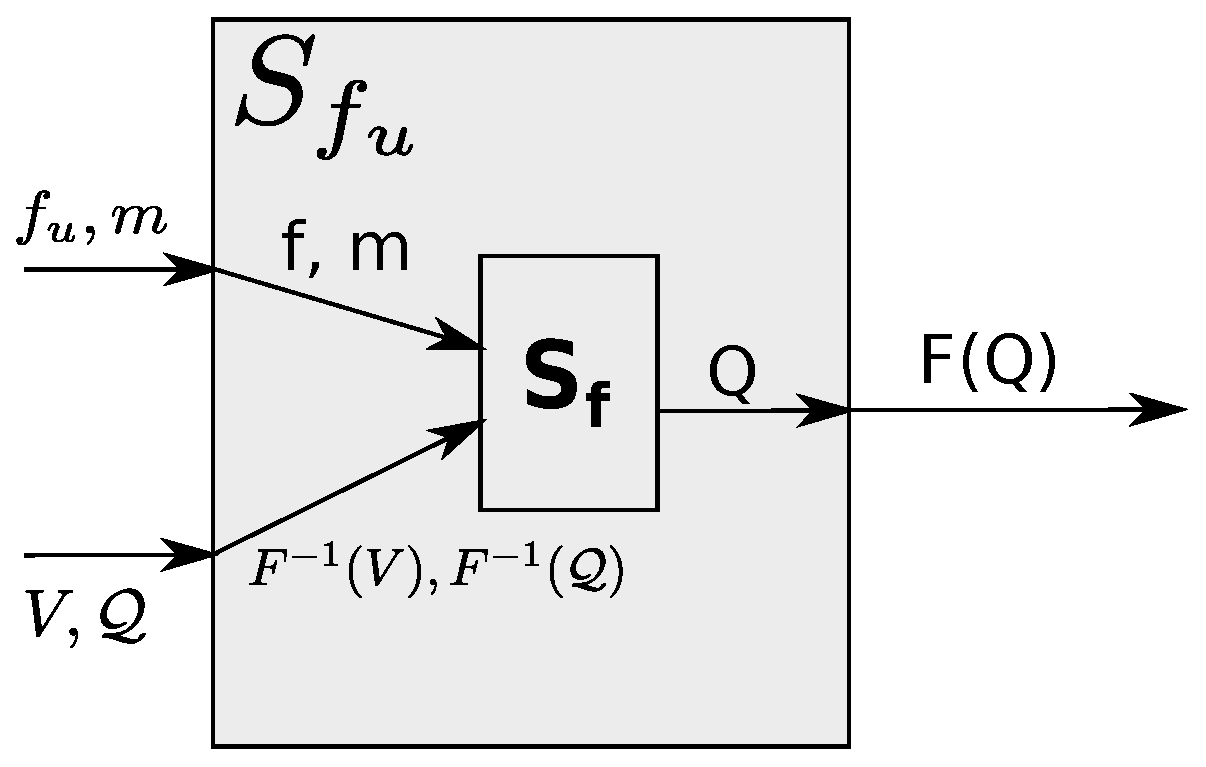
\includegraphics[width=.45\linewidth]{figures/S-f-to-u}
    \label{fig:S-t-to-u}
  }
  \caption{These two figures illustrate how to construct a strategy for an
    arbitrary PDF $f$ from one for the uniform distribution $f_u$, and vice versa.
Here, we depict a strategy as a box that takes four inputs $f, m, V,
  \mathcal Q$ (PDF, number of unknown values, reported values set, and set of asked
  queries) and returns $Q$ (the next query).} \label{fig:uniform}
\end{figure}

We next prove that descending query strategies, in which all bidders are
asked whether their valuations are above $a_i$ for a decreasing sequence of
$a_i$, are optimal.  (For a descending query strategy, as soon as we get a
positive reply, we are done, so the contingency plan does not need to branch.)

\begin{lemma}\label{lemma:descending}
Every optimal strategy 
uses only 
descending queries
$Q_1 = [a_1, 1), ~Q_2 = [a_2, a_1), ~Q_3 = [a_3, a_2)\ldots$
(with the possible exception of strategies that differ only on a measure
zero set
and are therefore equivalent to a descending-query strategy with
probability $1$).
\end{lemma}

\begin{proof}
Let us assume, for the sake of contradiction,
that there exists  an optimal strategy  that uses a 
non-descending query (meaning, one that differs from a descending query on
a non-measure-zero set).
In that strategy $S$, there must be a first non-descending query
$Q_{i+1} = S\big(F, m, V, \mathcal Q = \{Q_1, Q_2, \ldots, Q_i\}\big)$
% where
%$Q_1$ to $Q_i$ are all descending.  
Consider an alternative descending query
$Q'_{i+1} = [a'_{i+1}, a_i)$ (or $Q'_{i+1} = [a'_{i+1}, 1)$ if $i = 0$) such
that
\[
\Pr(v \in Q_{i+1}) = \int \limits_{Q_{i+1}} f(x) \mathrm d x = \int \limits_{Q'_{i+1}} f(x) \mathrm d x = \Pr(v \in Q'_{i+1})
\]
%(After $Q'_{i+1}$, we query optimally.)
%After $Q'_{i+1}$, we will use as optimal query as
%possible.

Because $Q_1$ to $Q_i$ are all descending, we have $m = n$ and $V = \emptyset$ (otherwise
an optimal strategy should terminate without asking $Q_{i+1}$).
Let $C$ be the expected cost of using $S$ from this point on
(starting with $Q_{i+1}$), and let $C'$ be the expected cost of 
of using $Q'_{i+1}$ and querying
optimally after that. We have\\
$
C = b + \sum_{j=0}^n p_j ( j \cdot c + C_j)
$
and
$
C' = b + \sum_{j=0}^n p'_j ( j \cdot c + C'_j)
$
where
%\begin{enumerate}
%\item 
$p_j$ (or $p'_j$) is the probability that there are $j$ reported values
within $Q_{i+1}$ (or $Q'_{i+1}$), and
%\item 
$C_j$ (or $C'_j$) is the expected cost of later queries given that $j$ values have been
found in $Q_{i+1}$ (or $Q'_{i+1}$).
%\end{enumerate}

Because $\Pr(v \in Q_{i+1}) = \Pr(v \in Q'_{i+1})$, we have $p'_j = p_j$
for all $j$.  We have $C_n = C'_n = 0$.
By Lemma~\ref{lemma:uniform},
$C_0 = C'_0 = C^*(n)$ 
because if we know that no value lies in $Q_1, Q_2, \ldots, Q_{i+1}$, the
remaining problem  is equivalent to that with the revised PDF
\[
f_{i+1}(x) = \begin{cases}
	\lambda f(x), & x \notin Q_1 \cup Q_2 \cup \ldots \cup Q_{i+1} \\
	0, & x \in Q_1 \cup Q_2 \cup \ldots \cup Q_{i+1}
\end{cases}
\]
where $\lambda$ is a constant that makes $\int_0^1 f_{i+1}(x) dx = 1$.
Finally, since $Q'_{i+1}$ is a descending query, for all $0 < j < n$,
$C'_j = 0$ but $C_j > 0$ (because for these values of $j$, it is possible
that all reported values in $Q_{i+1}$ lie below some value that has not
been queried yet).  Moreover, there exists some $j$ with $0 < j < n$ and
$p_j > 0$ unless (1) the probability of each agent's reply to $Q_{i+1}$ is
$1$---but in this case it differs only on a measure zero set from the
descending query that asks for all the remaining values, contradicting our
assumption; (2) the probability of each agent's reply to $Q_{i+1}$ is
$0$---but such a measure zero query is clearly suboptimal;
or (3) $n=1$---but in this case any query that differs by more
than a measure zero set from the query that asks for all the remaining
values is clearly suboptimal.
Hence, $C' < C$, contradicting our initial assumption.
\end{proof}

It follows that:

%vc: somewhere say something about having to query even when 1 bidder
%remains.  move up no-blind-allocation def and maybe refer to it in theorems

\begin{theorem}\label{theorem:MVA_eq}
Among all mechanisms
that are
required to allocate efficiently,
%(allocate the item to the bidder with highest
%valuation), 
Multi-round Vickrey Auctions (MVAs) are of minimum cost.
\end{theorem}

\begin{proof}
%The best case optimizing problem defined in definition \ref{def:query} provides
%us a lower bound of minimum cost we can achieve by any mechanisms.  
By Lemma~\ref{lemma:descending}, we can restrict our attention to
mechanisms with  descending query strategies
%such lower bound minimum cost can be achieved by
%descending query strategy 
$Q_1 = [a_1, 1], Q_2 = [a_2, a_1), Q_3 = [a_3, a_2) \ldots$.
For any such mechanism, Theorem~\ref{theorem:MVA_eq} tells us how to find reserve prices $r_1, r_2,
\ldots$ such that the corresponding MVA has a Bayes-Nash equilibrium that
is equivalent to this descending-query mechanism.
% any such mechanism is equivalent to the
%Bayes-Nash equilibrium of an MVA
%we are able to design such an MVA
%with reserve prices $r_1, r_2, \ldots$  whose Bayesian Nash Equilibrium
%achieves this best case descending query strategy.  Thus, MVAs are of minimum cost.
\end{proof}

By the revenue equivalence theorem,  we obtain that MVAs are optimal:

\begin{corollary}
If the bidders have no cost for bidding ($\beta_2=0$), MVAs 
that minimize cost for the seller
are optimal
among mechanisms that allocate efficiently.
%If all broadcast costs and bid costs are charged to sellers, MVAs are
%optimal if efficiency is required.  Such optimal MVA is the one that minimizes
%the overall cost.
\end{corollary}

\subsection{MVAs with Minimum Cost}
\label{sec:alpha-MVA}

The above analysis still leaves open what the optimal parameters
(thresholds $a_i$, or equivalently, reserve prices $r_i$) of the optimal
MVA are for a given setting $f, n, b, c$ (valuation PDF, number of bidders,
broadcast cost, bid cost).  According to Lemma~\ref{lemma:uniform}, the
cost does not depend on $f$ and it suffices to restrict our attention to
the uniform distribution.
Let $\rho = \frac{b}{c}$ (for cases where $c>0$).

%we can always derive an optimal mechanism for any
%$F$ from a uniform distribution.
% Thus we will focus on uniform cases
%below. 
%We will also introduce $\rho = \frac{b}{c}$ to simplify our analysis
%by normalize bid cost $c$ to $1$ and thus broadcast cost $b$ to $\rho$.

\begin{definition}
Given $f$, we define the $\alpha$-MVA to be the MVA in which in each round, the expected
number of nonsilent bids in that round (conditional on having reached that
round) is $(1-\alpha)n$.  In the case where $f$ is uniform, the
$\alpha$-MVA is characterized by $a_i = \alpha^i$.
\end{definition}

\begin{proposition}
For the purpose of minimizing total cost when $\beta_2=0$ under the constraint of efficient allocation:
If $c = 0$, the Vickrey auction (the $0$-MVA) is optimal.
If $\rho = b = 0$, the Dutch auction (which is approximated by the
$(1-\epsilon)$-MVA) is optimal.  
Otherwise, it is optimal to use an $\alpha$-MVA where $\alpha$ satisfies
$$\alpha^{n-1} (\rho + (1-\alpha)n) - (1-\alpha^n) = 0$$
%vc: unique solution??
\end{proposition}
\begin{proof}
If $c=0$, the Vickrey auction has cost $b$, which is optimal.
If $\rho=b=0$, the expected total cost of the Dutch auction is $c$ (since
with probability $1$ only one agent will reply), which is optimal.
For the remaining case, we first argue that there must be some $\alpha$-MVA
that is optimal.  
By  Lemma~\ref{lemma:uniform}, we can assume $f$ is uniform.
By Theorem~\ref{theorem:MVA_eq}, some MVA must be
optimal.  For this MVA, consider $a_1$.  If $a_i=0$, this is the
$0$-MVA. If $a_i>0$, then if at least one bidder is above $a_1$, we finish after
the first query; otherwise, the resulting conditional distribution for each
bidder is $f|_{[0,a_1)}$. According to Lemma~\ref{lemma:uniform}, we can
rescale this conditional distribution to the uniform distribution over
$[0,1)$ to arrive back at our original problem; and an optimal mechanism
for that is the same MVA that starts with query $a_1$ (which translates to
$a_1^2$ without rescaling).  Repeated application of this reasoning results
in the $\alpha$-MVA with $\alpha=a_1$.

All that remains to show is the characterization of this $\alpha$.
If $C_\alpha$ is the expected overall cost for the $\alpha$-MVA, then we
have $C_\alpha = b + (1-\alpha)nc + \alpha^n C_\alpha$, or equivalently 
$C_\alpha = \frac{b+(1-\alpha)nc }{ 1-\alpha^n}$.
If we optimize this with respect to $\alpha$, we must either have
\begin{align}\label{eq:alpha}
\frac{\partial C}{\partial \alpha} = \frac{{\alpha}^{n-1}\,n\,\left(
b+\left( 1-\alpha\right) \,nc\right) }{{\left( 1-{\alpha}^{n}\right)
}^{2}}-\frac{nc}{1-{\alpha}^{n}} &= 0 \nonumber\\
&\Updownarrow\nonumber\\
\alpha^{n-1} (\rho + (1-\alpha)n) - (1-\alpha^n) &= 0
\end{align}
%vc: double-check first equation (unnormalized)
or have $\alpha$ at a boundary value ($0$ or $1$). However, $\alpha=1$ (or
approaching $1$) is clearly suboptimal unless $b=0$, a case that we have
already covered; $\alpha=0$ can be ruled out because $\frac{\partial
  C}{\partial \alpha} |_{\alpha = 0} < 0$.
\end{proof}


%An optimal MVA must be an $\alpha$-MVA where each round only $(1-\alpha) n$
%bidders are expected to bid, i.e. $a_1 = \alpha, a_{i+1} = \alpha \cdot a_i$
%for uniform cases. Then the expected overall cost $C$ satisfies: $ C = \rho +
%(1-\alpha)n+\alpha^n C$. In the right hand side, the first term $\rho$ is the
%broadcast we have to use in the first round, the second term $(1-\alpha)n$ is
%the expected bid cost for the first round, the third term $\alpha^n C$ is
%a recursive term, the probability that no one bids times if that
%happens the same cost $C$ should be expected in later rounds.  

%From that equation, we get $C = \frac{
%\rho+(1-a)n }{ 1-\alpha^n }$. To minimize cost $C$, we either choose boundary
%cases $\alpha = 0, 1$ or we have: 

%\begin{align}\label{eq:alpha}
%\frac{\partial C}{\partial \alpha} = \frac{{\alpha}^{n-1}\,n\,\left(
%\rho+\left( 1-\alpha\right) \,n\right) }{{\left( 1-{\alpha}^{n}\right)
%}^{2}}-\frac{n}{1-{\alpha}^{n}} &= 0 \nonumber\\
%&\Updownarrow\nonumber\\
%\alpha^{n-1} (\rho + (1-\alpha)n) - (1-\alpha^n) &= 0
%\end{align}

%The boundary case $\alpha = 0$ can be ruled out because $\frac{\partial
%C}{\partial \alpha} |_{\alpha = 0} < 0$.
%%\footnote{As a result of $\alpha \neq 0$, optimal $\alpha$-MVA always has
%%infinite many rounds which seems to refine the result in [cite Increasing
%%Threshold Search] which claims it's either one round or infinite many rounds.
%%However, in their work, the total bid cost isn't necessarily linear with
%%the number of biddings. Thus it's a more general proof than our linear case.}  
%When $\alpha = 1$, $\alpha$-MVA becomes Dutch Auction thus $\rho$ must be $0$
%(otherwise total broadcast cost would be infinity). And this is indeed a
%solution of equation \ref{eq:alpha} when $\rho = 0$. Thus equation
%$\ref{eq:alpha}$ characterize the optimal $\alpha$ in all cases.

This result is analogous to a result by Sarne et
al.~\cite{SarneSR2010:IncreasingSearch}; translating\footnote{Sarne et
  al.~motivate their model as performing increasingly broad searches for an
  optimal agent and thereby focus on increasing threshold search to find a
  minimum, rather than decreasing queries to find a maximum.}
 their result into our
setting also gives a proof that $\alpha$-MVAs are optimal
among MVAs and also characterizes the optimal value of $\alpha$.  However, they do
not provide a proof that MVAs are optimal among all mechanisms; their setup
implicitly restricts attention to MVAs (when translated to our setting).
%vc: make sure last sentence is true. 


%Thus if they not
%intuitive please reference more details there.  Our simplified cost model
%(with efficiency constraint and no buyer's cost) is equivalent to their cost
%model where learning cost is linear to the number of replied agents.  That
%paper makes descending query as a contraint \footnote{In their model they want
%to find the minimum value so increasing threshold search is equivalent to
%descending query} and proves that $\alpha$-MVA is optimal among descending
%query mechanisms. Our focus in this section, however, is to have a preliminary
%introduction for MVA and proves optimality of descending queries and eventually
%MVAs. Thus we omit the proof about $\alpha$-MVA. Even for the $\alpha$, we will
%be more interested in its relation with larger $n$ so we will give
%approximations for $\alpha$.

\subsection{Approximation of $\alpha$}

\begin{figure*}
\centering
  \subfigure{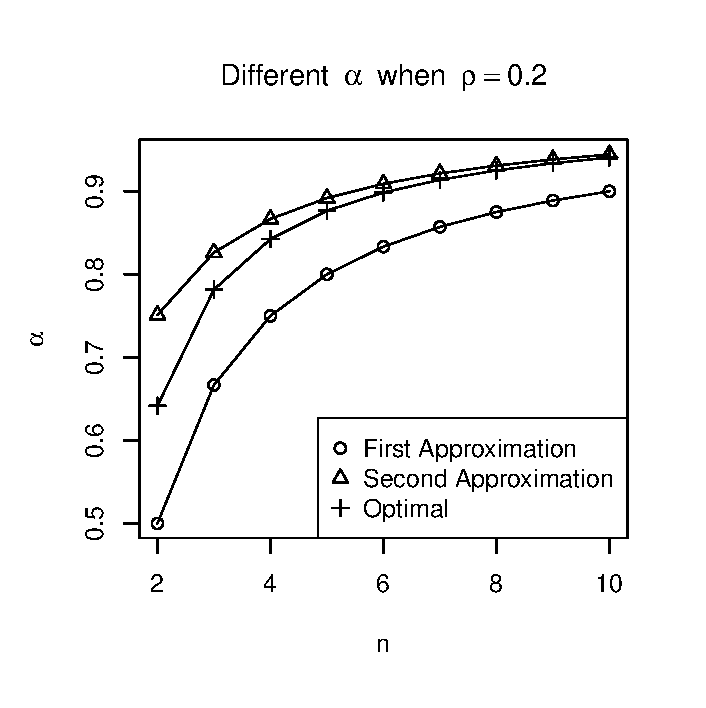
\includegraphics[trim=0 5mm 5mm 5mm, clip, width=.3\linewidth]{figures/alpha_when_rho0.20.eps}}
  \subfigure{\includegraphics[trim=0 5mm 5mm 5mm, clip, width=.3\linewidth]{figures/alpha_when_rho1.00.eps}}
  \subfigure{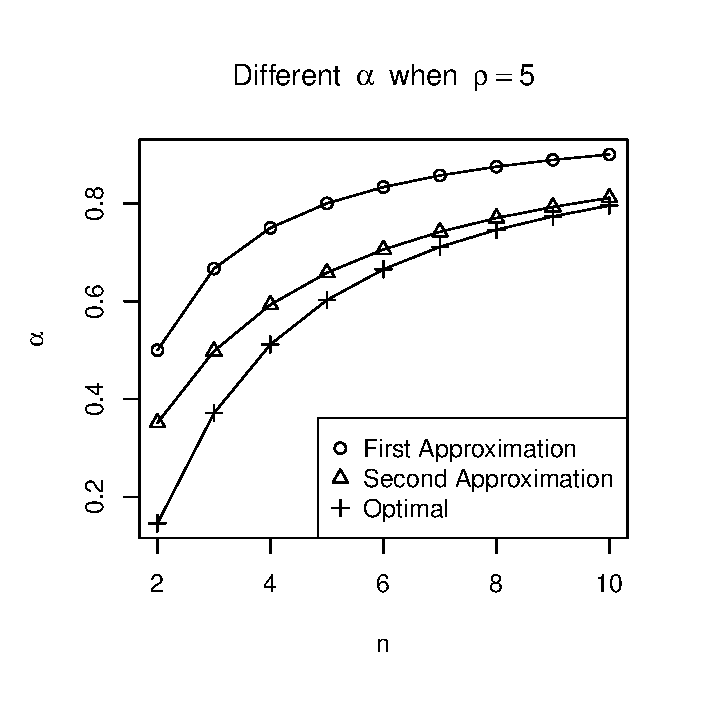
\includegraphics[trim=0 5mm 5mm 5mm, clip, width=.3\linewidth]{figures/alpha_when_rho5.00.eps}}
  \subfigure{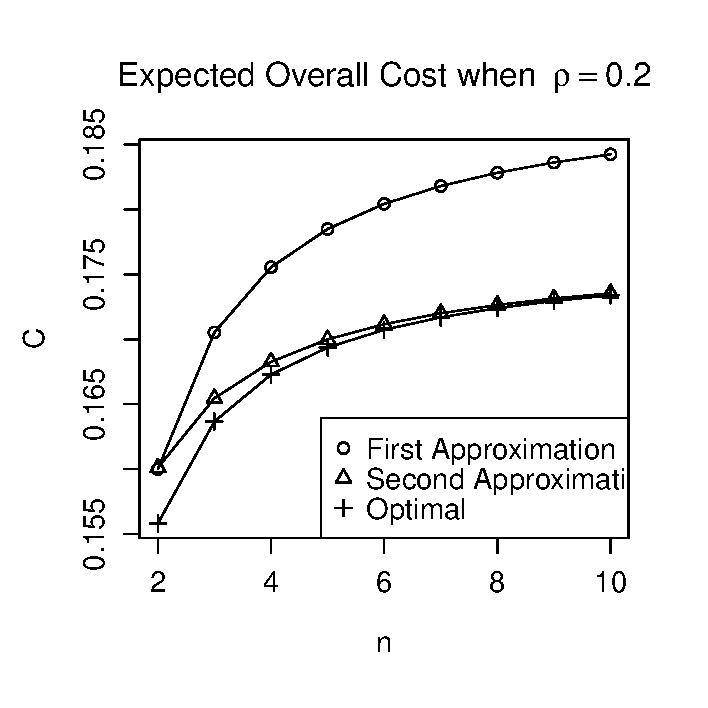
\includegraphics[trim=0 5mm 5mm 5mm, clip, width=.3\linewidth]{figures/C_when_rho0.20.eps}}
  \subfigure{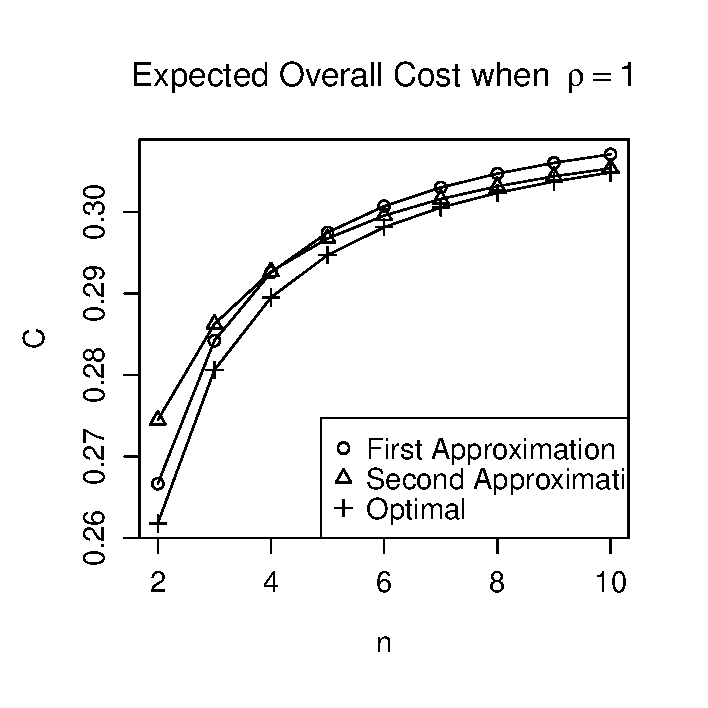
\includegraphics[trim=0 5mm 5mm 5mm, clip, width=.3\linewidth]{figures/C_when_rho1.00.eps}}
  \subfigure{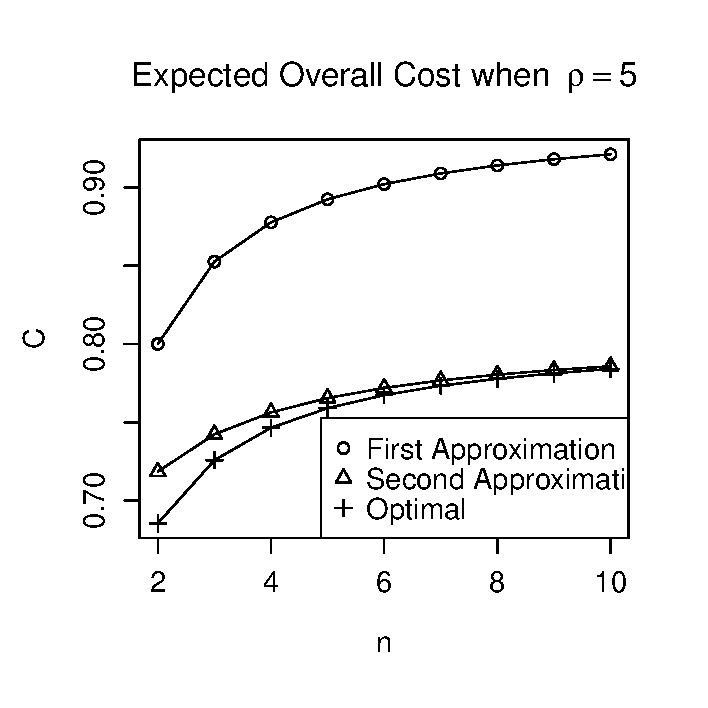
\includegraphics[trim=0 5mm 5mm 5mm, clip, width=.3\linewidth]{figures/C_when_rho5.00.eps}}
  \caption{Comparisons for optimal  $\alpha$ and its approximations. The first
  approximation is $\alpha = 1-1/n$, the second is $\alpha =
  (-W(-1-\rho))^{-1/n}$. The second row is the corresponding cost for different
  $\alpha$} 
  \label{fig:alpha}
\end{figure*}

It is difficult to get an exact closed formula for optimal $\alpha$ by equation
\ref{eq:alpha}. Thus we are going to use some simpler formulas to approximate
$\alpha$. We will conduct experiments to compare our approximation with the
optimal $\alpha$ that is computed numerically. 

Firstly, $\alpha = 1-1/n$ is a natural guess which means each round the
expected number of biddings is equal to $1$. It turns out to be quite good:

\begin{theorem}
$\alpha = 1-1/n$ is a $1/(1-e^{-1})$ approximation of optimal $\alpha$-MVA.
That means, by simply choosing $\alpha = 1-1/n$, we would at most get about
$1.582$ times of optimal cost. Another obersavation of this approximation is
that no matter how large $n$ is, the cost of this simple approximation is at
most $(\rho+1) / (1-e^{-1}) = O(1)$. Thus the optimal cost is bounded by
constant $O(1)$ no matter how large $n$ is.
\end{theorem}

\begin{proof}
$C(\alpha = 1-1/n) = (\rho+1)/(1-(1-1/n)^n)$. Because $(1-1/n)^n \leq e^{-1}$,
we have $C(\alpha = 1-1/n) \leq (\rho+1)/(1-e^{-1})$.  It is obvious that at
least one broadcast and one bidding is required to terminate so $C \geq
\rho+1$. This completes the proof.
\end{proof}

A better approximation when $n$ is large is to observe that $\alpha \rightarrow
1$ when $n$ grows large.  Thus we guess 
%\footnote{We tried several guesses and
%this is the one that finally turns out to work. Note that $(1-\alpha)n$ must be
%bounded (otherwise optimal cost won't be bounded by $O(1)$ as well) thus it's
%either a constant or a weird perturbation. It's natural to try constant first}
that $(1-a)n \approx A$ (for some constant $A$) and $\alpha^n \approx
\alpha^{n-1}$. Then we have: 
$$ n (\rho+A) \cdot \alpha^n - n(1-\alpha^n) = 0 $$ 
which gives us $\alpha = (1+\rho+A)^{-1/n}$. Put this back to $\lim_{n
\rightarrow \infty} (1-a)n = A$ we have $\ln (1+\rho+A) = A$ which gives us
\begin{align}\label{eq:approx2}
A = -1-\rho-W(-1-\rho)\nonumber\\
\alpha = (-W(-1-\rho))^{-1/n} 
\end{align}
where $W(x)$ is the Lambert W function [cite wikipedia?] defined by $W(x)
e^{W(x)} = x$. Actually, $w\,e^w = x$ has two solutions for $w$ when $-1 < x <
0$. Here our $W(x)$ refers to the lower\footnote{The upper branch is
$W_0(x) > -1$ when $-1 < x < 0$} branch $W_{-1}(x) < -1$. This
second approximation that converges to the optimal one when $n$ is large:

\begin{theorem}\label{theorem:approx1}
Suppose that the optimal $\alpha$ is $\alpha^*$ which
satisfies equation \ref{eq:alpha}. Then $\alpha = (-W(-1-\rho))^{-1/n}$ satisfies
$$\lim_{n \rightarrow \infty} C(\alpha^*) = \lim_{n \rightarrow \infty} C(\alpha = (-W(-1-\rho))^{-1/n})$$
That is, our approximation's cost will converge to optimal cost when $n$ grows to
infinity.
\end{theorem}

\begin{proof}
Define sequence $\alpha^*_n, C^*_n$ where $n = 1, 2, 3, \ldots$ to be sequences of
optimal $\alpha^*$ and corresponding optimal cost $C^*$ when there are $n$
bidders. We first show that $C^*_n$ is increasing: if we make
$(\alpha_{n-1})^{n-1} = (\alpha^*_n)^n$, then we have 1) The expected broadcast
cost of $\alpha_{n-1}$-MVA with $n-1$ bidders is equal to that of
$\alpha^*_n$-MVA with $n$ bidders as the probability that one round will
terminate is the same; 2) $\alpha_{n-1} < \alpha^*_n$ thus the expected bidding
cost of $\alpha_{n-1}$-MVA with $n-1$ bidders should be less than that of
$\alpha^*_n$-MVA with $n$ bidders. Therefore, $C^*_{n-1} \leq C_{n-1}(\alpha_{n-1}) < C^*_n$.
Thus sequence $C^*$ is indeed strictly increasing.

Secondly, theorem \ref{theorem:approx1} says $C^*_n$ is bounded. Therefore
$(1-\alpha^*)n$ must also be bounded otherwise $C = \frac{\rho+(1-\alpha)n}{1-\alpha^n}$ cannot be bounded.
Thus according to Bolzano-Weierstrass theorem [cite wikipedia?], there must be
a subsequence $\alpha^*_{n_i}$ such that $(1-\alpha^*_{n_i})n$ converges to some constant $A$.
Recall that $\alpha^*$ satisfies equation \ref{eq:alpha} and obviously $\lim_{n \rightarrow \infty} \alpha^* = 1$, 
we could use calculations similar to what we used for equation \ref{eq:approx2} to derive
\begin{align*}
&\lim_{n_i \rightarrow \infty} (1-\alpha^*_{n_i})n_i = A = -1-\rho-W(-1-\rho)\\
&\lim_{n_i \rightarrow \infty} (\alpha^*_{n_i})^{n_i} = \lim_{n_i \rightarrow \infty} (\alpha^*_{n_i})^{n_i-1} = (-W(-1-\rho))^{-1}
\end{align*}
This proves that
$$\lim_{n_i \rightarrow \infty} C(\alpha^*) = \lim_{n_i \rightarrow \infty} C(\alpha = (-W(-1-\rho))^{-1/n_i})$$
Then using the fact that $C^*_n$ is strictly increasing and bounded completes the proof.
\end{proof}

Experiments in figure \ref{fig:alpha} compare the optimal $\alpha$, our first approximation
of $\alpha = 1-1/n$ and our second approximation $\alpha = (-W(-1-\rho))^{-1/n}$
together with their corresponding cost under settings $\rho = 0.2, 1, 5$.

As figure \ref{fig:alpha} shows, the first approximation $1-1/n$ is bounded
to be a constant time of optimal cost while the second approximation converges to optimal
cost when $n$ grows large. When $\rho$ is close to $1$, both two
approximations are very close to the optimal one. But the second approximation is much better
when $\rho$ is much smaller or greater than $1$. Anyway, the second approximation is not always
better than the first approximation, as the case $\rho = 1, n = 2$ shows.

\subsection{Experiments}\label{sec:eff_experiment}
Now let us compare optimal $\alpha$-MVA with other kinds of MVA. In all
following experiments, the valuation distribution is always uniform over $[0,
1]$. According to lemma \ref{lemma:uniform}, other distributions can always be
adapted to uniform distribution so this will not be a problem.  Also recall that
under this simpler model, the revenue is fixed thus the profit is
completely determined by cost. Thus we will only compare cost.

$\alpha$-MVA can potentially have infinite many rounds. But in reality, it is
more naturaly to come up with an MVA that has finite many, say $k$ rounds at
most. Let us call them $k$-MVA where $k$ is some positive integers. One
particualr $k$- MVA is uniform $k$-MVA where the $k$ thresholds is uniformly
distributed over $[0, 1]$.  It is also known as fixed-step search strategy in
\cite{SarneSR2010:IncreasingSearch, DBLP:conf/iwdc/HassanJ04}. An optimal uniform MVA is the uniform
$k$-MVA that minimize the cost by choosing the best $k$.

In practice, such $k$ might also be very limited. For example, if someone need
to sell something in $3$ days before moving out, the $k$ might be limited to
$3$ since it is too annoying to send out two broadcast messages per day (e.g. it
might be labeled as spam by selling platform).  With this limitation, one can
still use uniform thresholds as a baseline. Or we may formulate this as another
optimzing problem and solve the best $k$ thresholds under this constraint (this
problem is defined and solved in section \ref{sec:general_analysis} and
equation \ref{eq:diff_C_general}).  Between the baseline $k$ uniform thresholds
and the optimal $k$ thresholds, another heurestic way to get $k$ thresholds is
to use $\alpha, \alpha^2, \ldots, \alpha^{k-1}$ as thresholds. That means, in
first $k-1$ rounds, we query as if we have infinite many rounds, and we query
all the left in last round. We call this mechanism as $\alpha$-cutoff-$k$-MVA.

The comparison results achieved from simulation experiments are shown in figure
\ref{fig:cost_comparisons}. Here are some observations:

\begin{figure*}
\centering
    \subfigure[$\rho = 0.5$]{
        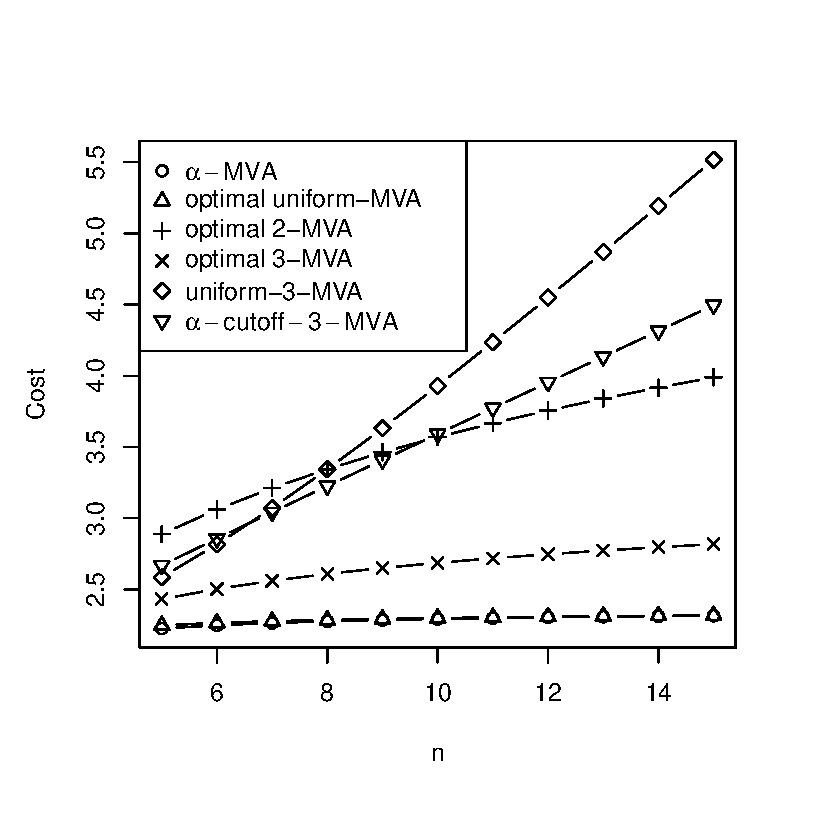
\includegraphics[trim=0 5mm 5mm 15mm, clip, width=.3\linewidth]{figures/analyze_cost_.5_5_15.eps}
        \label{fig:cost_comparison_.5}
    }
    \subfigure[$\rho = 2$]{
        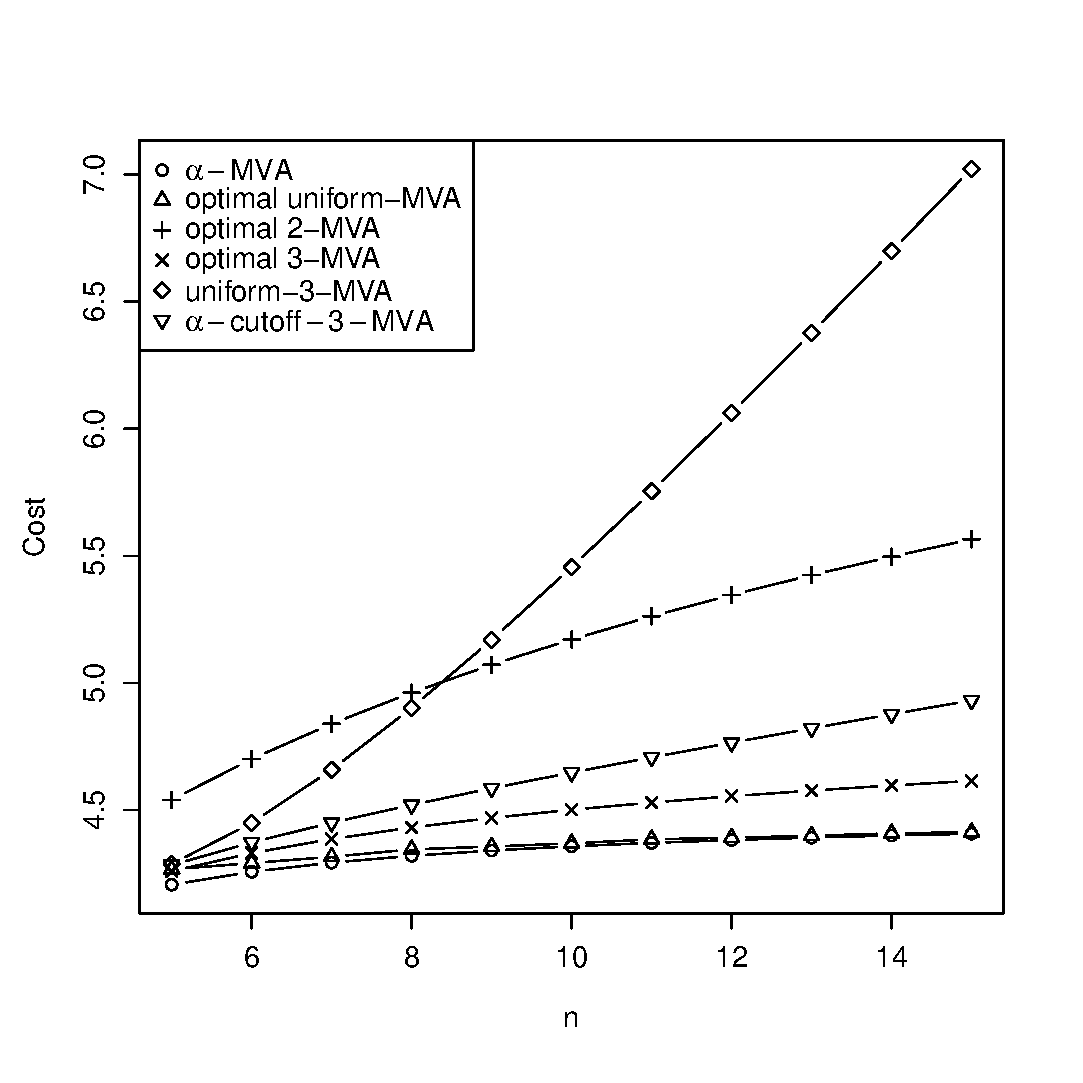
\includegraphics[trim=0 5mm 5mm 15mm, clip, width=.3\linewidth]{figures/analyze_cost_2_5_15.eps}
        \label{fig:cost_comparison_2}
    }
    \caption{Cost comparison for different MVAs over $n$, number of bidders, and $\rho$, broadcast/bid cost ratio.}
    \label{fig:cost_comparisons}
\end{figure*}

\begin{itemize}
\item The optimal uniform-MVA's cost is very close to optimal $\alpha$-MVA's,
especially when $n$ is large. That is probably because
    \begin{enumerate}
        \item $\alpha$ approaching $1$ when $n$ grows large, which makes the
        first $k$ thresholds $\alpha, \alpha^2, \alpha^3, \ldots, \alpha^k$
        close to uniform thresholds $1-(1-\alpha), 1-2(1-\alpha), \ldots,
        1-k(1-\alpha)$; 

        \item the probability that the highest value falls out of first $k$
        thresholds, $\alpha^{nk}$, becomes negligible for large $n$.
    \end{enumerate}

\item The optimal $k$-MVA's cost decreases and approaches to optimal cost quickly
when $k$ grows (check optimal $2$-MVA and $3$-MVA).

\item When $k$ is small, uniform thresholds has significant higher cost than optimal
$k$-MVA, and the heuristic $\alpha$-cutoff-$k$-MVA.

\item The heuristic $\alpha$-cutoff-$k$-MVA works pretty well especially when
$\rho$ is large as shown in figure \ref{fig:cost_comparison_.5}. But it is not
as good as optimal $2$-MVA when $\rho$ is small and $n$ is large as shown in
figure \ref{fig:cost_comparison_2}. Thus find the right thresholds is even more
important than adding one more round in those cases.

\end{itemize}
